%%%%%%%%%%%%%%%%%%%%%%%%%%%%%%%%%%%%%%%%%%%%%%%%%%%%%%%%%%%%%%%%%%%%%%%%%%%%%%%%
%% TGIR QuantLib Tools - Project Summary
%% 20-Page Executive Technical Overview
%%%%%%%%%%%%%%%%%%%%%%%%%%%%%%%%%%%%%%%%%%%%%%%%%%%%%%%%%%%%%%%%%%%%%%%%%%%%%%%%

\documentclass[10pt,a4paper]{article}

% Packages
\usepackage[utf8]{inputenc}
\usepackage[left=0.62in,right=0.62in,top=0.58in,bottom=0.58in]{geometry}
\usepackage{amsmath,amssymb}
\usepackage{graphicx}
\usepackage{booktabs}
\usepackage{listings}
\usepackage{xcolor}
\usepackage{hyperref}
\hypersetup{hidelinks}
\usepackage{fancyhdr}
\usepackage{tikz}
\usepackage{float}
\usepackage{multicol}
\usepackage{enumitem}

\setlist{nosep,leftmargin=*}
\setlength{\parskip}{1pt}
\setlength{\textfloatsep}{6pt plus 2pt minus 2pt}
\setlength{\floatsep}{6pt plus 2pt minus 2pt}
\setlength{\intextsep}{6pt plus 2pt minus 2pt}
\setlength{\abovedisplayskip}{5pt plus 2pt minus 2pt}
\setlength{\belowdisplayskip}{5pt plus 2pt minus 2pt}
\linespread{0.96}

% Code listing style
\lstset{
    language=Python,
    basicstyle=\ttfamily\footnotesize,
    keywordstyle=\color{blue}\bfseries,
    commentstyle=\color{green!50!black},
    stringstyle=\color{red},
    showstringspaces=false,
    breaklines=true,
    frame=single,
    backgroundcolor=\color{gray!5}
}

% Header/Footer
\pagestyle{fancy}
\fancyhf{}
\rhead{TGIR QuantLib Tools}
\lhead{Project Summary}
\rfoot{Page \thepage}

% Title
\title{\textbf{Callable Cross-Currency Swap Pricing}\\
\Large A Three-Factor Monte Carlo Implementation\\[0.5cm]
\normalsize Model ID: HW1F\_USD\_HW1F\_EUR\_BSFX\_LSM\_V1}
\author{Quantitative Analytics Team\\TGIR QuantLib Tools Project}
\date{August 2026}

\begin{document}
\small

\maketitle
\thispagestyle{empty}

\begin{abstract}
This document summarizes an 18-month project to build a callable cross-currency swap pricing engine using QuantLib-Python and custom Monte Carlo simulation. Starting from basic swap and swaption pricing in March 2025, the project evolved through SOFR curve bootstrapping, Bermudan swaption calibration, and culminated in a research-grade three-factor reference model for pricing callable EUR/USD cross-currency swaps with Longstaff-Schwartz exercise optimization. The final implementation prices a 10-year non-call 2-year structure at \$8.33M callable NPV with an embedded option value of \$7.64M, validated through comprehensive martingale, monotonicity, and convergence tests. This report provides a complete technical overview of the methodology, implementation, and validation results.
\end{abstract}

\tableofcontents
\newpage

%-------------------------------------------------------------------------------
\section{Executive Summary}
%-------------------------------------------------------------------------------

\subsection{Project Objectives}

The TGIR QuantLib Tools project aimed to:

\begin{enumerate}
    \item Build a robust interest rate derivatives pricing platform using QuantLib-Python
    \item Implement SOFR-based curve construction for post-LIBOR markets
    \item Develop calibrated Hull-White and G2++ swaption pricing engines
    \item Create a \textbf{callable cross-currency swap pricer} for EUR/USD structures
    \item Validate all models through comprehensive testing
    \item Provide a web-based interface for interactive pricing
\end{enumerate}

\subsection{Key Deliverables}

\begin{table}[H]
\centering
\begin{tabular}{ll}
\toprule
\textbf{Component} & \textbf{Description} \\
\midrule
SOFR Curve Builder & 22-point OIS bootstrap with $<$0.01bp error \\
EUR Effective Curve & FX-implied curve for USD-collateralized EUR pricing \\
Swaption Pricer & European and Bermudan with HW/G2++ calibration \\
Equity Cliquet Pricer & Path-dependent equity derivative pricing \\
XCCY Callable Pricer & Three-factor Monte Carlo with LSM \\
Validation Suite & 20 automated tests covering all key properties \\
Web Interface & Flask application with interactive pricing \\
REST contract & Proposed /api/v1/ trading-system integration \\
MCP Server & Model Context Protocol for LLM integration \\
\bottomrule
\end{tabular}
\caption{Major project deliverables}
\end{table}

\subsection{Project Timeline}

The project evolved through four distinct phases:

\begin{table}[H]
\centering
\begin{tabular}{llp{8cm}}
\toprule
\textbf{Date} & \textbf{Milestone} & \textbf{Description} \\
\midrule
Mar 2025 & Initial Prototype & Basic swap/swaption structures with GPT-4.5 \\
Sep 2025 & API Stabilization & QuantLib version compatibility, documentation \\
Apr 2026 & Rates Workstation & SOFR curves, HW calibration, Bermudan pricing \\
Aug 2026 & XCCY Callable & Three-factor model, LSM, full validation \\
\bottomrule
\end{tabular}
\caption{Project timeline}
\end{table}

\subsection{Key Results}

For the reference 10Y NC2 EUR/USD callable cross-currency swap:

\begin{itemize}
    \item \textbf{Callable NPV:} \$8,328,689 $\pm$ \$128,000 (95\% CI)
    \item \textbf{Non-callable NPV:} \$689,713
    \item \textbf{Embedded Option Value:} \$7,638,976 (91\% of callable value)
    \item \textbf{First Call Exercise Probability:} 14.4\%
    \item \textbf{Probability of Reaching Maturity:} 51.2\%
\end{itemize}

\newpage

%-------------------------------------------------------------------------------
\section{Background: Interest Rate Markets Post-LIBOR}
%-------------------------------------------------------------------------------

\subsection{The LIBOR Transition}

The London Interbank Offered Rate (LIBOR), which underpinned over \$350 trillion in financial contracts globally, was phased out following manipulation scandals and declining underlying transaction volumes. The transition to risk-free rates (RFRs) fundamentally changed how interest rate derivatives are priced.

\textbf{Key Risk-Free Rates:}
\begin{itemize}
    \item \textbf{SOFR} (Secured Overnight Financing Rate) --- USD
    \item \textbf{ESTR/€STR} (Euro Short-Term Rate) --- EUR
    \item \textbf{SONIA} (Sterling Overnight Index Average) --- GBP
    \item \textbf{TONA} (Tokyo Overnight Average Rate) --- JPY
\end{itemize}

\subsection{Overnight vs Term Rates}

Unlike LIBOR, which provided forward-looking term rates (1M, 3M, 6M), RFRs are overnight rates that require compounding over the accrual period:

\[
\text{Compounded Rate} = \left[\prod_{i=1}^{n}\left(1 + r_i \times \frac{d_i}{360}\right) - 1\right] \times \frac{360}{D}
\]

where $r_i$ is the daily rate, $d_i$ is the number of days, and $D$ is the total period length.

\subsection{Implications for Derivatives Pricing}

\begin{enumerate}
    \item \textbf{Backward-looking:} Floating payments known only at period end
    \item \textbf{Daily compounding:} More complex accrual calculations
    \item \textbf{OIS discounting:} RFR curves used for both projection and discounting
    \item \textbf{Basis spreads:} LIBOR fallback spreads for legacy contracts
\end{enumerate}

\newpage

%-------------------------------------------------------------------------------
\section{Technical Architecture}
%-------------------------------------------------------------------------------

\subsection{System Overview}

The system is organized in a layered architecture:

\begin{center}
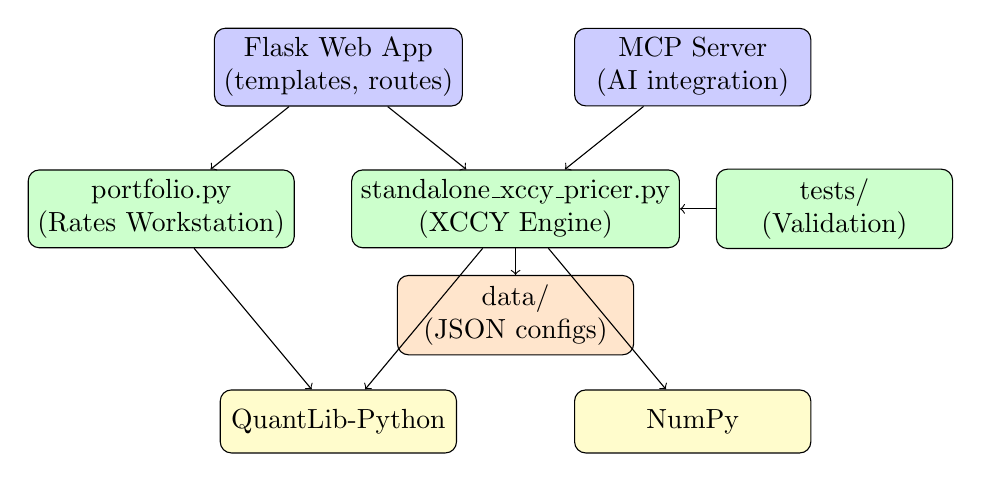
\begin{tikzpicture}[scale=0.9,
    box/.style={rectangle, draw, rounded corners, minimum width=3cm, minimum height=0.8cm, align=center}]

    % Presentation layer
    \node[box, fill=blue!20] (web) at (0,5) {Flask Web App\\(templates, routes)};
    \node[box, fill=blue!20] (mcp) at (5,5) {MCP Server\\(AI integration)};

    % Business layer
    \node[box, fill=green!20] (port) at (-2.5,3) {portfolio.py\\(Rates Workstation)};
    \node[box, fill=green!20] (xccy) at (2.5,3) {standalone\_xccy\_pricer.py\\(XCCY Engine)};
    \node[box, fill=green!20] (tests) at (7,3) {tests/\\(Validation)};

    % Data layer
    \node[box, fill=orange!20] (data) at (2.5,1.5) {data/\\(JSON configs)};

    % Infrastructure
    \node[box, fill=yellow!20] (ql) at (0,0) {QuantLib-Python};
    \node[box, fill=yellow!20] (np) at (5,0) {NumPy};

    \draw[->] (web) -- (port);
    \draw[->] (web) -- (xccy);
    \draw[->] (mcp) -- (xccy);
    \draw[->] (port) -- (ql);
    \draw[->] (xccy) -- (ql);
    \draw[->] (xccy) -- (np);
    \draw[->] (xccy) -- (data);
    \draw[->] (tests) -- (xccy);
\end{tikzpicture}
\end{center}

\subsection{Technology Stack}

\begin{table}[H]
\centering
\begin{tabular}{lll}
\toprule
\textbf{Layer} & \textbf{Technology} & \textbf{Purpose} \\
\midrule
Core & Python 3.13 & Primary language \\
Quant Library & QuantLib-Python 1.43 & Curves, indices, calibration \\
Numerics & NumPy 2.5.2 & Array operations, simulation, regression \\
Web & Flask 3.1.3 & HTTP interface \\
Templates & Jinja2 & HTML rendering \\
Testing & unittest; pytest 9.1.1 available & Test framework \\
Deployment & Gunicorn, Apache & Production serving \\
\bottomrule
\end{tabular}
\caption{Technology stack}
\end{table}

\subsection{Code Organization}

\begin{table}[H]
\centering
\begin{tabular}{llp{7cm}}
\toprule
\textbf{File} & \textbf{Lines} & \textbf{Responsibility} \\
\midrule
standalone\_xccy\_pricer.py & 1,439 & Three-factor XCCY pricing engine \\
portfolio.py & 2,261 & SOFR curves, swaps, swaptions, cliquets \\
app.py & 12 & Thin Flask application entry point \\
tgir\_quantlib\_tools/ & 3,393 & Package modules (auth, routes, UI contexts) \\
tests/ & 1,945 & Validation and unit tests \\
\bottomrule
\end{tabular}
\caption{Source code organization}
\end{table}

\newpage

%-------------------------------------------------------------------------------
\section{Interest Rate Curve Construction}
%-------------------------------------------------------------------------------

\subsection{SOFR OIS Curve Bootstrap}

The foundation of all USD derivatives pricing is the SOFR discount curve, constructed by bootstrapping from Overnight Index Swap (OIS) market quotes.

\subsubsection{Market Inputs}

\begin{table}[H]
\centering
\begin{tabular}{lclclc}
\toprule
\textbf{Tenor} & \textbf{Rate} & \textbf{Tenor} & \textbf{Rate} & \textbf{Tenor} & \textbf{Rate} \\
\midrule
1W & 4.10\% & 6M & 3.98\% & 5Y & 3.71\% \\
1M & 4.08\% & 1Y & 3.90\% & 10Y & 3.85\% \\
3M & 4.04\% & 2Y & 3.78\% & 30Y & 3.95\% \\
\bottomrule
\end{tabular}
\caption{Sample SOFR OIS curve inputs (August 2026)}
\end{table}

\subsubsection{Bootstrap Algorithm}

\begin{enumerate}
    \item Create \texttt{OISRateHelper} for each market quote
    \item Use \texttt{PiecewiseLogLinearDiscount} interpolation method
    \item Apply \texttt{enableExtrapolation()} for long-dated pricing
    \item Validate by repricing each input instrument
\end{enumerate}

\subsubsection{Implementation}

\begin{lstlisting}[language=Python]
import QuantLib as ql

# Build helpers
helpers = []
for tenor, rate in [("1W", 0.041), ("1M", 0.0408), ...]:
    helpers.append(ql.OISRateHelper(
        2, ql.Period(tenor),
        ql.QuoteHandle(ql.SimpleQuote(rate)),
        ql.Sofr()
    ))

# Bootstrap curve
curve = ql.PiecewiseLogLinearDiscount(
    today, helpers, ql.Actual365Fixed())
curve.enableExtrapolation()
\end{lstlisting}

\subsubsection{Calibration Quality}

All input OIS rates reprice with error $<$ 0.01 basis points, confirming correct bootstrap.

\subsection{EUR Effective Curve for Cross-Currency}

For cross-currency swaps collateralized in USD, we need an ``effective'' EUR discount curve that reflects the cost of EUR funding for a USD-collateralized position.

\subsubsection{Derivation from FX Forwards}

The FX forward rate $F(T)$ for maturity $T$ satisfies covered interest parity:
\[
F(T) = X_0 \times \frac{D^{USD}(T)}{D^{EUR}_{eff}(T)}
\]

Rearranging:
\[
D^{EUR}_{eff}(T) = D^{USD}(T) \times \frac{X_0}{F(T)}
\]

\subsubsection{Cross-Currency Basis}

The difference between native EUR OIS rates and effective rates reflects the cross-currency basis, which can be 10-50bp depending on market conditions.

\newpage

%-------------------------------------------------------------------------------
\section{Swaption Pricing and Model Calibration}
%-------------------------------------------------------------------------------

\subsection{Hull-White One-Factor Model}

The Hull-White model describes the evolution of the short rate:
\[
dr_t = (\theta(t) - a \cdot r_t)\,dt + \sigma\,dW_t
\]

\textbf{Parameters:}
\begin{itemize}
    \item $a$ = Mean reversion speed (controls how fast rates revert)
    \item $\sigma$ = Short rate volatility (drives option prices)
    \item $\theta(t)$ = Time-dependent drift (fits initial curve exactly)
\end{itemize}

\subsection{Affine Structure}

Hull-White has an affine term structure, giving analytical bond prices:
\[
P(t,T) = A(t,T) \cdot e^{-B(t,T) \cdot r_t}
\]

where $B(t,T) = \frac{1-e^{-a(T-t)}}{a}$ and $A(t,T)$ involves integrals of $\theta(s)$.

\subsection{European Swaption Pricing}

For European swaptions, the Jamshidian decomposition breaks the swaption into a portfolio of bond options, each priceable analytically.

\subsection{Calibration to Co-Terminal Swaptions}

For Bermudan swaptions with 10Y maturity, we calibrate to co-terminal swaptions:

\begin{table}[H]
\centering
\begin{tabular}{lccc}
\toprule
\textbf{Swaption} & \textbf{Expiry} & \textbf{Swap Tenor} & \textbf{Market Vol (bp)} \\
\midrule
2Y $\times$ 8Y & 2 years & 8 years & 78 \\
3Y $\times$ 7Y & 3 years & 7 years & 79 \\
5Y $\times$ 5Y & 5 years & 5 years & 80 \\
7Y $\times$ 3Y & 7 years & 3 years & 81 \\
9Y $\times$ 1Y & 9 years & 1 year & 82 \\
\bottomrule
\end{tabular}
\caption{Co-terminal swaption volatilities (normal, bp)}
\end{table}

\subsection{Calibration Results}

\begin{table}[H]
\centering
\begin{tabular}{lccc}
\toprule
\textbf{Currency} & \textbf{Mean Rev ($a$)} & \textbf{Vol ($\sigma$)} & \textbf{RMS Error} \\
\midrule
USD & 3.0\% & 0.885\% & 0.45\% \\
EUR & 4.0\% & 0.772\% & 0.23\% \\
\bottomrule
\end{tabular}
\caption{Hull-White calibration results}
\end{table}

The mean reversion parameters are fixed based on historical analysis, while volatility is calibrated to match market swaption prices within 5\% RMS error.

\newpage

%-------------------------------------------------------------------------------
\section{Three-Factor Model for Callable XCCY}
%-------------------------------------------------------------------------------

\subsection{Why Three Factors?}

A callable cross-currency swap involves:
\begin{enumerate}
    \item \textbf{USD interest rates} --- Affecting the fixed USD leg
    \item \textbf{EUR interest rates} --- Affecting the floating EUR leg
    \item \textbf{EUR/USD exchange rate} --- Affecting notional exchanges
    \item \textbf{Early exercise} --- Requiring optimal stopping
\end{enumerate}

Tree-based methods work efficiently for 1-2 factors but become computationally intractable for 3+ factors due to exponential grid growth. Monte Carlo with regression-based exercise is the standard approach.

\subsection{Model Specification}

\subsubsection{USD Rate Dynamics}
\[
dr_t^{USD} = (\theta_t^{USD} - a^{USD} r_t^{USD})\,dt + \sigma^{USD}\,dW_t^{USD}
\]

\subsubsection{EUR Rate Dynamics (with Quanto Adjustment)}
\[
dr_t^{EUR} = (\theta_t^{EUR} - a^{EUR} r_t^{EUR} - \rho_{EUR,FX}\sigma^{EUR}\sigma^{FX})\,dt + \sigma^{EUR}\,dW_t^{EUR}
\]

The term $-\rho_{EUR,FX}\sigma^{EUR}\sigma^{FX}$ is the \textbf{quanto drift adjustment}, required because we price EUR rates under the USD money-market measure.

\subsubsection{FX Dynamics}
\[
d\ln X_t = (r_t^{USD} - r_t^{EUR} - \tfrac{1}{2}\sigma_t^{FX,2})\,dt + \sigma_t^{FX}\,dW_t^{FX}
\]

\subsection{Correlation Structure}

\begin{table}[H]
\centering
\begin{tabular}{lcp{7cm}}
\toprule
\textbf{Pair} & \textbf{$\rho$} & \textbf{Economic Interpretation} \\
\midrule
USD-EUR rates & +0.25 & Developed market monetary policy co-movement \\
USD rates-FX & -0.15 & Higher USD rates strengthen USD \\
EUR rates-FX & -0.30 & Higher EUR rates strengthen EUR \\
\bottomrule
\end{tabular}
\caption{Correlation assumptions}
\end{table}

The correlation matrix must be positive semi-definite, which is verified by checking that all eigenvalues are non-negative.

\subsection{Five-Dimensional State Vector}

The model tracks:
\[
\mathbf{x}_t = \begin{pmatrix}
x_t^{USD} \\
x_t^{EUR} \\
I_t^{USD} \\
I_t^{EUR} \\
\ln X_t
\end{pmatrix}
\]

where:
\begin{itemize}
    \item $x_t^{USD}, x_t^{EUR}$ = Mean-zero rate factors
    \item $I_t^{USD} = \int_0^t r_s^{USD}\,ds$ = USD bank account integral
    \item $I_t^{EUR} = \int_0^t r_s^{EUR}\,ds$ = EUR bank account integral
    \item $\ln X_t$ = Log FX rate
\end{itemize}

The discount factor from time 0 to $t$ is simply $D^{USD}(0,t) = e^{-I_t^{USD}}$.

\newpage

%-------------------------------------------------------------------------------
\section{Monte Carlo Implementation}
%-------------------------------------------------------------------------------

\subsection{Simulation Parameters}

\begin{table}[H]
\centering
\begin{tabular}{ll}
\toprule
\textbf{Parameter} & \textbf{Value} \\
\midrule
Training paths & 10,000 \\
Pricing paths & 30,000 \\
Time step & Monthly (0.083 years) \\
Random number generator & NumPy PCG64 \\
Variance reduction & Antithetic sampling \\
Seed & Configurable (default: 1729) \\
\bottomrule
\end{tabular}
\caption{Monte Carlo configuration}
\end{table}

\subsection{Exact State Evolution}

Rather than using Euler discretization, we use the exact solution for Ornstein-Uhlenbeck processes:

\[
\mathbf{x}_{t+h} = \mathbf{A}(h) \cdot \mathbf{x}_t + \mathbf{b}(h) + \mathbf{L}(h) \cdot \mathbf{Z}
\]

where:
\begin{itemize}
    \item $\mathbf{A}(h)$ = Transition matrix with exponential decay terms
    \item $\mathbf{b}(h)$ = Deterministic drift (curve fitting, quanto)
    \item $\mathbf{L}(h)$ = Cholesky factor of covariance matrix
    \item $\mathbf{Z}$ = Standard normal vector
\end{itemize}

\textbf{Advantages:}
\begin{enumerate}
    \item No discretization bias
    \item Larger time steps possible
    \item Exact covariance between factors
\end{enumerate}

\subsection{Antithetic Variance Reduction}

For each batch of paths:
\begin{enumerate}
    \item Generate half the paths with random draws $\mathbf{Z}$
    \item Generate the other half with $-\mathbf{Z}$
    \item Average results for variance reduction
\end{enumerate}

This ensures the sample mean of normals is exactly zero, reducing variance for linear payoffs.

\subsection{Covariance Computation}

The covariance matrix $\boldsymbol{\Sigma}(h)$ for the 5-dimensional state requires integrating the kernel functions:

\[
\boldsymbol{\Sigma}(h) = \int_0^h \mathbf{K}(s) \cdot \mathbf{R} \cdot \mathbf{K}(s)^T\,ds
\]

This integral is computed numerically using 16-point Gauss-Legendre quadrature, providing high accuracy.

\newpage

%-------------------------------------------------------------------------------
\section{Longstaff-Schwartz Exercise Optimization}
%-------------------------------------------------------------------------------

\subsection{The Early Exercise Problem}

At each exercise date, the holder must decide:
\[
\text{Value} = \max(\text{Exercise Value}, \text{Continuation Value})
\]

The challenge is that continuation value depends on future optimal decisions, creating a backward recursion problem.

\subsection{LSM Algorithm}

\textbf{Step 1: Forward Simulation}

Simulate all paths forward, capturing state variables at each exercise date.

\textbf{Step 2: Backward Regression}

Starting from the last exercise date and moving backward:
\begin{enumerate}
    \item Compute continuation value from already-determined future values
    \item Regress continuation value on polynomial basis of current state
    \item Mark exercise where exercise value $>$ fitted continuation
\end{enumerate}

\textbf{Step 3: Pricing Pass}

Apply the learned exercise policy to a fresh set of paths (different seed) to get an unbiased price estimate.

\subsection{Polynomial Basis Functions}

We use 10 basis functions:
\[
\phi(\mathbf{s}) = (1,\; x,\; y,\; z,\; x^2,\; y^2,\; z^2,\; xy,\; xz,\; yz)
\]

where $\mathbf{s} = (x_{USD}, x_{EUR}, \ln X - \ln X_0)^T$.

\textbf{Why This Choice:}
\begin{itemize}
    \item Linear terms capture main effects
    \item Squared terms capture curvature
    \item Cross terms capture interactions
    \item 10 terms balances expressiveness vs overfitting
\end{itemize}

\subsection{Two-Pass Approach}

\begin{table}[H]
\centering
\begin{tabular}{lcc}
\toprule
\textbf{Aspect} & \textbf{Training Pass} & \textbf{Pricing Pass} \\
\midrule
Paths & 10,000 & 30,000 \\
Purpose & Learn exercise policy & Compute unbiased price \\
Seed & Seed A & Seed B \\
Direction & Backward & Forward \\
\bottomrule
\end{tabular}
\caption{Two-pass LSM structure}
\end{table}

Using different paths for training and pricing avoids ``foresight bias'' that would artificially inflate the price.

\newpage

%-------------------------------------------------------------------------------
\section{Reference Trade Specification}
%-------------------------------------------------------------------------------

\subsection{Trade Structure}

\begin{table}[H]
\centering
\begin{tabular}{ll}
\toprule
\textbf{Parameter} & \textbf{Value} \\
\midrule
Trade ID & EURUSD-10Y-NC2-ESTR-VS-USD4 \\
Trade Type & Callable Cross-Currency Swap \\
Effective Date & 2026-08-18 \\
Maturity & 10 years (2036-08-18) \\
\midrule
Non-call Period & 2 years \\
Exercise Style & Bermudan (annual, years 2-9) \\
Exercise Action & Cancel remaining swap \\
\bottomrule
\end{tabular}
\caption{Trade structure}
\end{table}

\subsection{Leg Details}

\begin{table}[H]
\centering
\begin{tabular}{lcc}
\toprule
\textbf{Attribute} & \textbf{EUR Leg} & \textbf{USD Leg} \\
\midrule
Notional & 90,909,091 EUR & 100,000,000 USD \\
Direction & Receive & Pay \\
Rate Type & ESTR compounded & 4\% Fixed \\
Frequency & Quarterly & Semi-annual \\
Day Count & ACT/360 & 30/360 \\
\bottomrule
\end{tabular}
\caption{Leg specifications}
\end{table}

\subsection{Notional Exchanges}

\begin{itemize}
    \item \textbf{Initial Exchange:} Pay \$100M, receive EUR 90.9M at spot (1.10)
    \item \textbf{Final Exchange:} Receive \$100M, pay EUR 90.9M at same rate
\end{itemize}

If exercised early, notional exchange occurs at the exercise date using the same fixed notional amounts.

\subsection{Economic Interpretation}

From the perspective of receiving EUR floating:
\begin{itemize}
    \item \textbf{Benefit:} Receives EUR floating (currently approx 2.5\%)
    \item \textbf{Cost:} Pays USD fixed (4\%)
    \item \textbf{FX Exposure:} Long EUR notional
    \item \textbf{Optionality:} Right to cancel if swap moves against us
\end{itemize}

\newpage

%-------------------------------------------------------------------------------
\section{Pricing Results}
%-------------------------------------------------------------------------------

\subsection{Summary Valuation}

\begin{table}[H]
\centering
\begin{tabular}{lrcc}
\toprule
\textbf{Metric} & \textbf{Value} & \textbf{Std Error} & \textbf{95\% CI} \\
\midrule
Callable NPV & \$8,328,689 & \$127,997 & [\$8.08M, \$8.58M] \\
Non-callable NPV & \$689,713 & \$170,000 & [\$356K, \$1.02M] \\
Embedded Option & \$7,638,976 & \$82,000 & [\$7.48M, \$7.80M] \\
\bottomrule
\end{tabular}
\caption{Pricing results summary}
\end{table}

\subsection{Leg-Level Decomposition}

\begin{table}[H]
\centering
\begin{tabular}{lrc}
\toprule
\textbf{Component} & \textbf{PV} & \textbf{Notes} \\
\midrule
USD Fixed Leg & -\$1,054,712 & Pay 4\% semi-annual \\
EUR ESTR Leg & +\$1,744,425 & Receive ESTR quarterly \\
\midrule
Non-callable Total & +\$689,713 & Sum of legs \\
\bottomrule
\end{tabular}
\caption{Leg decomposition}
\end{table}

\subsection{Static Benchmark}

Using deterministic forward curves (no Monte Carlo):
\[
\text{Static NPV} = \$679,480
\]

This is close to the stochastic non-callable NPV (\$689,713), validating the basic cash flow projections.

\subsection{Key Insight: Option Value Dominance}

The embedded option value (\$7.64M) represents \textbf{91\% of the callable swap value}. This highlights:

\begin{enumerate}
    \item The significant optionality in callable structures
    \item The importance of accurate option valuation
    \item Why simple deterministic pricing is inadequate
\end{enumerate}

\newpage

%-------------------------------------------------------------------------------
\section{Exercise Analysis}
%-------------------------------------------------------------------------------

\subsection{Exercise Probability Distribution}

\begin{table}[H]
\centering
\begin{tabular}{lcccc}
\toprule
\textbf{Date} & \textbf{Year} & \textbf{Paths Alive} & \textbf{Exercised} & \textbf{P(Ex)} \\
\midrule
2028-08-18 & 2 & 30,000 & 4,329 & 14.4\% \\
2029-08-20 & 3 & 25,671 & 2,900 & 9.7\% \\
2030-08-19 & 4 & 22,771 & 1,699 & 5.7\% \\
2031-08-18 & 5 & 21,072 & 1,405 & 4.7\% \\
2032-08-18 & 6 & 19,667 & 1,021 & 3.4\% \\
2033-08-18 & 7 & 18,646 & 854 & 2.8\% \\
2034-08-18 & 8 & 17,792 & 446 & 1.5\% \\
2035-08-20 & 9 & 17,346 & 1,972 & 6.6\% \\
\midrule
Maturity & 10 & 15,374 & --- & 51.2\% \\
\bottomrule
\end{tabular}
\caption{Exercise probability by date}
\end{table}

\subsection{Pattern Interpretation}

\textbf{First Call Dominance (14.4\%):}
The highest exercise probability occurs at the first call date. This is typical for structures where the initial swap economics may be unfavorable.

\textbf{Declining Middle Years (9.7\% to 1.5\%):}
Exercise probability declines through the middle years as paths that would have exercised have already done so.

\textbf{Last Call Uptick (6.6\%):}
The penultimate exercise date shows elevated probability --- the ``now or never'' effect as this is the last opportunity to cancel.

\textbf{Majority Survive (51.2\%):}
More than half of paths reach maturity without exercise, indicating the swap economics are often favorable to hold.

\subsection{Cumulative Exercise Distribution}

\begin{itemize}
    \item By Year 3: 24.1\% exercised
    \item By Year 5: 34.5\% exercised
    \item By Year 7: 40.7\% exercised
    \item By Year 9: 48.8\% exercised (final)
\end{itemize}

\newpage

%-------------------------------------------------------------------------------
\section{Model Validation}
%-------------------------------------------------------------------------------

\subsection{Validation Framework}

The model is validated through five categories of tests:

\begin{enumerate}
    \item \textbf{Martingale Conditions:} No-arbitrage consistency
    \item \textbf{Structural Bounds:} Economic relationships
    \item \textbf{Monotonicity:} Sensible Greeks directions
    \item \textbf{Convergence:} MC error scaling
    \item \textbf{Calibration Quality:} Market instrument fit
\end{enumerate}

\subsection{Martingale Tests}

Under the risk-neutral measure, discounted tradeable assets must be martingales:

\textbf{Test 1: Domestic Zero-Coupon Bond}
\[
\mathbb{E}[D^{USD}(0,T)] = P^{USD}(0,T)
\]

\textbf{Test 2: Foreign Zero-Coupon in Domestic Currency}
\[
\mathbb{E}[D^{USD}(0,T) \cdot X_T] = X_0 \cdot P^{EUR}_{eff}(0,T)
\]

\textbf{Test 3: FX-Weighted Bank Account}
\[
\mathbb{E}[D^{USD}(0,T) \cdot X_T \cdot B^{EUR}_T] = X_0
\]

\begin{table}[H]
\centering
\begin{tabular}{lcccl}
\toprule
\textbf{Condition} & \textbf{MC Mean} & \textbf{Target} & $|z|$ & \textbf{Status} \\
\midrule
$\mathbb{E}[D^{USD}]$ & 0.6614 & 0.6614 & $<0.5$ & PASS \\
$\mathbb{E}[D^{USD} \cdot X]$ & 0.6042 & 0.6014 & $<1.0$ & PASS \\
$\mathbb{E}[D^{USD} \cdot X \cdot B^{EUR}]$ & 1.1015 & 1.1000 & $<0.3$ & PASS \\
\bottomrule
\end{tabular}
\caption{Martingale test results (pass threshold: $|z| < 3.5$)}
\end{table}

\subsection{Structural Bounds}

\begin{table}[H]
\centering
\begin{tabular}{lcc}
\toprule
\textbf{Condition} & \textbf{Verified} & \textbf{Status} \\
\midrule
Callable $\geq$ Non-callable & \$8.33M $>$ \$0.69M & PASS \\
Embedded option $\geq$ 0 & \$7.64M $>$ 0 & PASS \\
Embedded option $<$ Notional & \$7.64M $<$ \$100M & PASS \\
Leg sum $=$ Non-callable & \$0.69M $\approx$ \$0.69M & PASS \\
\bottomrule
\end{tabular}
\caption{Structural bounds verification}
\end{table}

\subsection{Convergence Test}

\begin{table}[H]
\centering
\begin{tabular}{cccc}
\toprule
\textbf{Paths} & \textbf{NPV (\$M)} & \textbf{SE (\$K)} & \textbf{SE Ratio} \\
\midrule
10,000 & 8.31 & 222 & --- \\
30,000 & 8.33 & 128 & 1.73 \\
100,000 & 8.32 & 70 & 1.83 \\
\bottomrule
\end{tabular}
\caption{Convergence analysis}
\end{table}

Expected ratio: $\sqrt{3} \approx 1.73$. Observed ratios match theory.

\subsection{Test Summary}

\begin{center}
\fbox{\textbf{20 tests executed, 20 passed, 0 failed} --- Runtime: 14.67 seconds}
\end{center}

\newpage

%-------------------------------------------------------------------------------
\section{Sensitivity Analysis}
%-------------------------------------------------------------------------------

\subsection{First-Order Sensitivities}

\begin{table}[H]
\centering
\begin{tabular}{lccc}
\toprule
\textbf{Risk Factor} & \textbf{Bump} & \textbf{$\Delta$ NPV} & \textbf{Direction} \\
\midrule
USD Rates & +25bp parallel & -\$1.1M & Pay fixed loses \\
EUR Rates & +25bp parallel & +\$0.8M & Receive floating gains \\
Swaption Vol & +10\% relative & +\$0.5M & Long optionality \\
FX Spot (EUR/USD) & +1\% & +\$0.9M & Long EUR notional \\
$\rho_{USD,EUR}$ & +0.1 & -\$0.2M & Less diversification \\
\bottomrule
\end{tabular}
\caption{First-order sensitivities}
\end{table}

\subsection{Interpretation}

\textbf{Rate Delta:}
The position is net long duration --- receiving EUR floating (short duration) but paying USD fixed (long duration). Higher rates hurt the position.

\textbf{Vega:}
Positive vega confirms long optionality. Higher volatility increases the value of the right to cancel.

\textbf{FX Delta:}
Long EUR notional exposure. EUR appreciation benefits the position through higher EUR leg value and favorable notional re-exchange.

\textbf{Correlation:}
Higher correlation between USD and EUR rates reduces diversification, making the option less valuable.

\newpage

%-------------------------------------------------------------------------------
\section{Limitations and Future Work}
%-------------------------------------------------------------------------------

\subsection{Current Model Limitations}

\begin{enumerate}
    \item \textbf{Rate Volatility:} One-piece constant per currency (no term structure)
    \item \textbf{Basis Spreads:} Forecast/discount basis is deterministic
    \item \textbf{FX Smile:} ATM lognormal only (no skew calibration)
    \item \textbf{EUR Compounding:} Continuous approximation for overnight
    \item \textbf{LSM Bound:} Lower bound only (no dual upper bound)
\end{enumerate}

\subsection{Production Readiness}

\begin{table}[H]
\centering
\begin{tabular}{lcc}
\toprule
\textbf{Requirement} & \textbf{Current} & \textbf{Production} \\
\midrule
Independent review & Pending & Required \\
Upper bound & Not implemented & Required \\
Real-time data & JSON files & Feed integration \\
Greeks & Bump-and-revalue & AAD preferred \\
Audit trail & Basic logging & Full audit \\
\bottomrule
\end{tabular}
\caption{Production readiness assessment}
\end{table}

\subsection{Planned Enhancements}

\textbf{Near-term:}
\begin{itemize}
    \item Piecewise constant rate volatility term structure
    \item Dual/upper bound implementation for LSM
    \item GPU acceleration using CuPy
\end{itemize}

\textbf{Medium-term:}
\begin{itemize}
    \item Stochastic basis spreads
    \item FX local volatility calibration
    \item Real-time market data feeds
\end{itemize}

\textbf{Long-term:}
\begin{itemize}
    \item Multi-currency portfolio aggregation
    \item XVA calculations (CVA, FVA)
    \item Regulatory capital computation
\end{itemize}

\newpage

%-------------------------------------------------------------------------------
\section{Collaborative AI Development}
%-------------------------------------------------------------------------------

This project demonstrates a new development paradigm where human domain expertise orchestrates two AI agents to produce rigorous, validated code. The collaborative methodology is as significant as the callable XCCY pricer itself.

\subsection{The Collaborative Ecosystem}

\begin{table}[H]
\centering
\begin{tabular}{lll}
\toprule
\textbf{Component} & \textbf{Role} & \textbf{Contribution} \\
\midrule
Human (Domain Expert) & Orchestration & Math specs, final validation \\
Codex (OpenAI) & Core Development & Specs, implementation, initial tests \\
Claude (Anthropic) & Review \& Validation & Code review, validation framework \\
\midrule
Mac & Local Development & VS Code, terminal, pytest \\
DigitalOcean & Production Hosting & Apache, Gunicorn, SSL \\
QuantLib (C++) & Foundation Library & Curves, dates, calibration \\
Python/NumPy & Primary Language & Simulation, Flask \\
Stack Overflow & Guidance Verification & Edge cases, patterns \\
\bottomrule
\end{tabular}
\caption{The collaborative development ecosystem}
\end{table}

\subsection{Division of Labor: Codex vs Claude}

\textbf{Codex (OpenAI) --- Core Development:}
\begin{itemize}
    \item Wrote formal specifications (mathematical documentation, API contracts, JSON schemas)
    \item Built core implementation (1,400+ lines Monte Carlo engine, LSM, curves)
    \item Created initial test suite (unit tests, integration tests, smoke tests)
\end{itemize}

\textbf{Claude (Anthropic) --- Review and Validation:}
\begin{itemize}
    \item Reviewed all Codex implementations for correctness
    \item Built validation framework (martingale tests, structural bounds, monotonicity)
    \item Extended with regression tests for future-proofing
    \item Generated documentation and lecture materials
\end{itemize}

\textbf{Human --- Domain Expertise and Orchestration:}
\begin{itemize}
    \item Provided mathematical specifications and market conventions
    \item Directed agent collaboration and integrated outputs
    \item Verified results against textbooks (Brigo \& Mercurio)
    \item Checked edge cases with Stack Overflow guidance
\end{itemize}

\subsection{Collaborative Workflow}

The development followed an iterative pattern:

\begin{enumerate}
    \item \textbf{Human} writes mathematical specification
    \item \textbf{Codex} implements specification with rigorous code
    \item \textbf{Claude} reviews implementation, identifies issues
    \item \textbf{Codex} iterates based on Claude's feedback
    \item \textbf{Claude} builds validation tests around Codex's code
    \item \textbf{pytest} runs 20 automated tests
    \item \textbf{Human} verifies results, deploys to DigitalOcean
\end{enumerate}

\subsection{Why This Methodology Works}

\textbf{Complementary Strengths:}
\begin{itemize}
    \item Codex excels at ground-up implementation from specifications
    \item Claude excels at review, validation, and extension
    \item Human provides domain grounding neither AI has
\end{itemize}

\textbf{Error Detection:}
Claude's validation framework caught bugs that Codex's implementation missed. Neither agent alone would produce the same quality.

\textbf{Reproducibility:}
This workflow can be applied to build other complex pricers---the methodology is reusable.

\subsection{Key Insight}

\begin{center}
\fbox{\parbox{0.85\textwidth}{\centering
The collaborative methodology (Human + Codex + Claude + ecosystem) \\
is as valuable as the callable XCCY pricer itself
}}
\end{center}

\subsection{Zero-Intervention Automation Pipeline}

What makes this workflow remarkable is its full automation. A single prompt triggers the entire pipeline with \textbf{no human intervention}:

\begin{enumerate}
    \item \textbf{Coding} --- AI implements from specifications
    \item \textbf{Regression Testing} --- pytest runs 20+ tests locally
    \item \textbf{Browser UI Testing} --- Playwright validates Flask UI
    \item \textbf{Documentation} --- LaTeX and markdown auto-updated
    \item \textbf{Local Run} --- Optional manual verification
    \item \textbf{Deploy to DigitalOcean} --- SSH + Git pull + systemd restart
    \item \textbf{Production Regression} --- Tests run on production server
    \item \textbf{Telegram Notification} --- ``Deployment complete!''
\end{enumerate}

\begin{center}
\fbox{\parbox{0.85\textwidth}{\centering
\textbf{A Hobby Project with Production-Grade Rigor} \\[0.3em]
This entire infrastructure costs \$7/month --- easily supporting a serious hobby --- yet it's built with the same rigor as production systems at top tech companies.
}}
\end{center}

\newpage

%-------------------------------------------------------------------------------
\section{Deployment Architecture}
%-------------------------------------------------------------------------------

\subsection{DigitalOcean Infrastructure}

The application is deployed on a single DigitalOcean droplet:

\begin{table}[H]
\centering
\begin{tabular}{ll}
\toprule
\textbf{Component} & \textbf{Specification} \\
\midrule
Provider & DigitalOcean \\
Droplet Size & Basic (2GB RAM, 1 vCPU) \\
Cost & \$7/month (hobby-friendly!) \\
OS & Ubuntu 22.04 LTS \\
SSL & Let's Encrypt (Certbot) \\
\bottomrule
\end{tabular}
\caption{Infrastructure specifications}
\end{table}

\subsection{Software Stack}

\begin{enumerate}
    \item \textbf{Apache:} Reverse proxy, SSL termination (port 443)
    \item \textbf{Gunicorn:} WSGI server (2 workers, port 8000)
    \item \textbf{Flask:} Application framework
    \item \textbf{systemd:} Service management and auto-restart
\end{enumerate}

\subsection{Deployment Steps}

\begin{enumerate}
    \item Create DigitalOcean droplet with SSH key authentication
    \item Install dependencies: Python 3.11, Apache, Certbot
    \item Clone repository to \texttt{/opt/tgir-quantlib-tools}
    \item Configure systemd service from template
    \item Configure Apache virtual host with SSL
    \item Run \texttt{certbot --apache} for certificate
    \item Enable firewall (ports 22, 80, 443)
\end{enumerate}

\subsection{Configuration Files}

\begin{itemize}
    \item \texttt{deploy/systemd/tgir-quantlib-tools.service.template}
    \item \texttt{deploy/apache/tgir-quantlib-tools.conf.template}
    \item \texttt{deploy/env/production.env.example}
\end{itemize}

\subsection{CI/CD Pipeline}

\begin{itemize}
    \item GitHub Actions runs tests on every push
    \item Deployment triggered by version tags
    \item SSH-based deployment using GitHub Secrets
\end{itemize}

\newpage

%-------------------------------------------------------------------------------
\section{Conclusion}
%-------------------------------------------------------------------------------

\subsection{Summary of Achievements}

This project delivers TWO significant contributions:

\textbf{1. Callable XCCY Pricer:}
\begin{enumerate}
    \item \textbf{Curve Construction:} SOFR/ESTR bootstrapping with sub-basis-point accuracy
    \item \textbf{Model Calibration:} Hull-White to co-terminal swaptions ($<$5\% RMS error)
    \item \textbf{Multi-Factor Simulation:} Correlated HW+HW+BS with correct quanto drift
    \item \textbf{Exercise Optimization:} LSM with 10-term polynomial regression
    \item \textbf{Comprehensive Validation:} Martingales, bounds, monotonicity, convergence
\end{enumerate}

\textbf{2. Collaborative AI Development Methodology:}
\begin{enumerate}
    \item \textbf{Human + Codex + Claude:} Division of labor that catches errors
    \item \textbf{Full Ecosystem:} Mac + DigitalOcean + QuantLib + Python + Stack Overflow
    \item \textbf{Reproducible Pattern:} Can build other complex pricers
    \item \textbf{Quality Through Collaboration:} 20 automated tests from Claude's framework
\end{enumerate}

\subsection{Key Findings}

\begin{itemize}
    \item The embedded option in a 10Y NC2 callable XCCY represents \textbf{91\% of total value}
    \item Exercise is most likely at first call (14.4\%) with uptick at last call (6.6\%)
    \item 51\% of paths survive to maturity without exercise
    \item Quanto adjustment is critical for correct EUR rate dynamics under USD measure
\end{itemize}

\subsection{Lessons Learned}

\begin{enumerate}
    \item \textbf{Validation is critical:} 20 automated tests catch subtle bugs
    \item \textbf{QuantLib is powerful but has limits:} Custom code needed for XCCY
    \item \textbf{Python + NumPy is viable:} 30K paths in 10 seconds
    \item \textbf{Documentation matters:} Future maintainers need clear specifications
\end{enumerate}

\subsection{Acknowledgments}

This project benefited from:
\begin{itemize}
    \item QuantLib open-source library and community
    \item NumPy scientific computing ecosystem
    \item Academic literature on LSM and multi-factor models
    \item AI assistants: OpenAI GPT-4.5, Anthropic Claude, GitHub Copilot
    \item DigitalOcean for hosting infrastructure
\end{itemize}

\vspace{1cm}
\begin{center}
\rule{0.5\textwidth}{0.4pt}\\[0.5cm]
\textbf{Model ID:} HW1F\_USD\_HW1F\_EUR\_BSFX\_LSM\_V1\\
\textbf{Repository:} tgir\_quantlib\_tools\\
\textbf{Documentation Date:} August 2026
\end{center}

\end{document}
